\chapter{Revisión de la literatura}\label{cap: EstadoArte}

En este capítulo se revisa el estado actual de la literatura en cuanto a problemas de Big Optimization se refiere, en concreto los \textbf{benchmarks} más utilizados en esta rama. Análogamente, una revisión del la literatura relacionada con el benchmark del EEG se llevará a cabo, prestando especial atención a las dos vertientes sobre las que se basa este estudio: las \textbf{técnicas previamente aplicadas} para resolver el problema del EEG y las propuestas más relevantes de la literatura actual en cuanto a \textbf{algoritmos de optimización de miles de variables} se refiere, donde intervienen técnicas de distinta naturaleza, con el objetivo final de establecer el símil sobre el que se basa el desarrollo de este Trabajo Fin de Grado. 

\section{CEC y Benchmarks}

Los problemas de optimización  han estado presentes desde los inicios de la computación evolutiva y una vertiente de estos, los \textbf{problemas de optimización de miles de variables (LSGO)}, se encuentra actualmente en auge dada la necesidad de resolución de problemas del mundo real donde la formulación de estos incurre en una representación con miles de variables que precisa de una optimización efectiva y eficiente.

\textbf{IEEE}, la organización profesional para el avance tecnológico más grande del mundo, ha sido desde 1999 la encargada de organizar el \textbf{Congress on Evolutionary Computation}, uno de las mayores y más importantes convenciones de computación evolutiva a nivel mundial \cite{IEEECEC}; en ella se exponen numerosas técnicas para resolver diversos problemas de optimización, siendo estas técnicas evaluadas a través de distintas competiciones, y donde la dimensionalidad del problema normalmente no supone un impedimento adicional a la hora de resolver los problemas que en ella se plantean.

Sin embargo, no es hasta el año 2008 cuando se propone la primera \textbf{Special Session \& Competition on Large-Scale Global Optimization}\cite{CEC-LSGO}, con el objetivo de establecer una base sobre la que evaluar las distintas propuestas, algoritmos o técnicas destinadas a resolver\textbf{ problemas de optimización de alta dimensionalidad}, donde las técnicas disponibles en ese momento sufrían una considerable reducción de su rendimiento conforme aumentaba el tamaño del espacio de soluciones.

A partir de este momento entran en escena un \textbf{conjunto de problemas de optimización representados por funciones acotadas} que, a diferencia de años anteriores, contenía un elevado número de variables a optimizar. Este conjunto de funciones se agrupa dentro de lo que se denomina un \textbf{benchmark} o \textbf{test suite} que sirve para evaluar el desempeño de las técnicas de tipo LSGO. El concepto de benchmark, tanto la propuesta original como el de alta dimensionalidad, será ampliado posteriormente en el capítulo \ref{cap:DisenioExp} donde se explicará en profundidad todo lo relacionado con el método para evaluar los algoritmos y técnicas que se proponen en las competiciones.

\section{\textit{EEG Problem} y propuestas de solución}

En el año 2015, durante el IEEE Congress on Evolutionary Computation llevado a cabo en Sendai, Japón\cite{IEEE-CEC2015}, se presenta la  \textbf{Optimization of Big Data 2015 Competition}\cite{CompetitionBigOpt} donde, a diferencia de otros años, no se propone un conjunto de funciones benchmark de alta dimensionalidad sino un problema completamente distinto, el de la \textbf{optimización de los datos de un electroencefalograma}, que ha sido descrito en el capítulo anterior.

No se conocen con exactitud todas las técnicas propuestas para esta competición, pero tras ésta los organizadores publican el artículo \textit{Evolutionary Big Optimization (Big Opt) of Signals}\cite{EvolutionaryBigOpt}, en el que se recogen los resultados obtenidos al aplicar el problema sobre dos técnicas evolutivas multiobjetivo consideradas como las más potentes: MOEA/D y NSGA-II.

\textbf{MOEA/D}\cite{MOEA/D} emplea la estrategia de descomposición para hacer frente a los problemas multiobjetivo: descompone el problema MO en un subconjunto de problemas y los optimiza de forma separada utilizando únicamente la información de los subproblemas vecinos, reduciendo considerablemente la complejidad del problema en cada generación si lo comparamos con el algoritmo \textbf{Nondominated Sorting GA II} (NSGA-II)\cite{NSGA-II}, que posee una complejidad de orden $O(MN^2)$ siendo \textit{M} la cantidad de objetivos y \textit{N} el tamaño de la población; el algoritmo crea una \textit{mating pool} donde la población de padres y offsprings se combinan, eligiendo posteriormente el mejor de estos, dando solución a los impedimentos típicos de los algoritmos MO que utilizan clasificación no-dominada.

En el artículo mencionado anteriormente, se propone el enfoque \textbf{multiobjetivo}, optimizando por separado ambas funciones \ref{eq:function1} y \ref{eq:function2}. Se elige optimizar dos representaciones distintas, frente al \textbf{dominio del tiempo} y al \textbf{de la frecuencia}; este último para intentar superar los inconvenientes derivados de la dimensionalidad del problema.

Los resultados muestran un mejor desempeño de \textbf{MOEA/D} frente a NSGA-II en la representación frente al dominio de la frecuencia, dado que esta, a través de una \textbf{Fast Fourier Transform} aplicada sobre los componentes principales, es capaz de reducir \textbf{hasta la mitad la dimensionalidad} del problema (con una frecuencia de 1Hz). La \textbf{reducción de la dimensionalidad} y los\textbf{ buenos resultados} conseguidos son las principales bazas a tener en cuenta de cara a una aplicación real donde los datos de un EEG sean procesados y posteriormente ``blanqueados" por algoritmos evolutivos multiobjetivo.

\subsection{MAGA-BigOpt: Algoritmo Genético Multi-Agente para optimización uniobjetivo}

\textbf{MAGA-BigOpt}, \textbf{\textit{A Multi-Agent Genetic Algorithm for Big Optimization Problems}}\cite{MAGA-BigOpt}, es la principal propuesta de solución para el problema del EEG formulado en la Optimization of Big Data 2015 Competition, con enfoque uniobjetivo. Esta técnica, basada en el framework MAGA\cite{MAGA}, ``\textit{reestructura los operadores de competición y autoaprendizaje, que finalmente combina con operadores de cruce y mutación para \textbf{simular la cooperación, competición y comportamientos de aprendizaje de los agentes}}".

MAGA, en primera instancia propuesto para optimización numérica global a gran escala en\cite{MAGA}, evolucionó para resolver el problema en cuestión, EEG, con 4 operadores genéticos donde un operador de autoaprendizaje con subgradiente es su principal activo, obteniendo resultados que superan con creces los propuestos como base en la competición mencionada.

Este algoritmo se basa en la idea de \textbf{agente}, que no es más que una solución candidata, y la \textbf{energía de un agente} computada como el valor negativo de la función $f$ definida en la ecuacion \ref{eq:FObj}. Los agentes se encuentran en un entorno similar a una rejilla $L$, que se llama la \textbf{rejilla de agente}, con tamaño $L_{size}\times L_{size}$. La representación vectorial de un agente (solución) permite situarlo en una posición $L_{i,j}$ donde tendrá 4 vecinos espaciales subyacentes: arriba, abajo, izquierda o derecha según donde se encuentre en la rejilla. 

El objetivo consiste por tanto en maximizar la energía de los agentes a través de los operadores evolutivos propuestos, donde los procesos de competición y cooperación son llevados a cabo por los \textbf{operadores de competición y cruce de vecinos} respectivamente, mientras que el uso del conocimiento del contexto se basa en los operadores de cruce y autoaprendizaje. La descripción completa de cada uno de los operadores y su aplicación se puede consultar en \cite{MAGA-BigOpt}.

Atendiendo a los resultados obtenidos tras aplicar MAGA-BigOpt sobre el problema del EEG, tanto en problemas con ruido como sin este, se observan valores superiores a los propuestos como base en la competición, alcanzando valores muy cercanos a cero y con una varianza prácticamente despreciable, hecho que junto a la potencia de los operadores propuestos, reafirma la candidatura de esta técnica a ser considerada como \textbf{punto de referencia} en este estudio tanto a niveles de calidad de la solución como a restricciones de tiempo, al elegir utilizar el mismo enfoque, uniobjetivo, por el que se ha optado en este trabajo.

\section{Algoritmos Large Scale Global Optimization} \label{cap:revisionLSGO}

Los computación evolutiva a través de algoritmos dedicados a la resolución de \textbf{problemas de optimización global continua con miles de variables} es un campo que, como anteriormente ha sido mencionado, ha sufrido una reciente evolución en cuanto al número de propuestas debido a la necesidad de plantear soluciones efectivas y sobre todo eficientes a una gran cantidad de problemas reales que pueden ser representados mediante un problema de Big Optimization.

La \textit{Special Session and Competition on Large-Scale Global Optimization} del WCCI 2018\cite{WCCI-SHADEILS} indica que no es hasta el año 2015 cuando se experimenta un cambio significativo entre la cantidad de artículos publicados en esta materia y los propuestos únicamente para conferencias; así lo refleja el gráfico de la figura \ref{fig:LSGO-Evolution}, donde se pueden ver los resultados que arroja la búsqueda del término ``\textit{Large Scale Global Optimization}"\ en la base de datos Scopus\cite{SCOPUS}, sitio desde el que se han obtenido la gran mayoría de referencias bibliográficas que se encuentran en este trabajo.

Un estudio publicado en 2014 bajo el nombre de \textbf{\textit{A comprehensive comparison of large scale global optimizers}}\cite{ComprehensiveComparison} recoge la comparativa entre las \textbf{tres mejores propuestas} de las sesiones del CEC 2010, CEC 2012, CEC 2013 y SOCO 2011 con el objetivo de \textbf{analizar el desempeño global} de aquellas técnicas cuando son evaluadas con respecto a\textbf{ tres distintos benchmarks} con distintos tipos de funciones, para determinar no solo la efectividad y eficiencia de forma individual sino también de manera global. Resaltar que los algoritmos que sean seleccionados para formar parte de este estudio serán detallados en profundidad en el capítulo \ref{cap:Analisis}.

\begin{figure}[h]
	\centering
	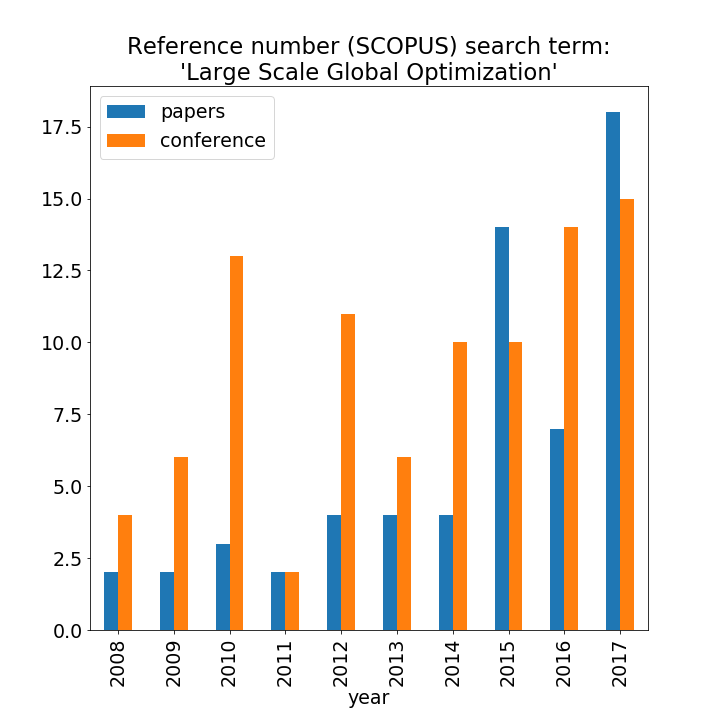
\includegraphics[scale=0.5]{imagenes/LSGO-Evolution}
	\caption{Evolución de las referencias de propuestas de algoritmos LSGO. Fuente: \cite{WCCI-SHADEILS}}
	\label{fig:LSGO-Evolution}
\end{figure}

\subsection{SOCO 2011 Special Issue}
La \textit{SOCO 2011 Special Issue} cuenta con fuertes propuestas como lo son \textbf{\textit{A MOS-based dynamic memetic differential evolution algorithm for continuous optimization: a scalability test}}\cite{MOS2010}, o MOS-SOCO2011, un algoritmo que basándose en la utilización del framework MOS (Multiple Offspring Sampling), es capaz de \textbf{combinar distintas estrategias de búsqueda} sin tener ninguna fuga; se combinan en este caso un algoritmo de \textbf{evolución diferencial (DE)} y la primera de las tres búsquedas locales del algoritmo MTS\cite{MTS-LSGO}, la \textbf{MTS-LS1}.

Ajustando la participación de cada técnica en base a una función de participación híbrida que favorece la utilización de aquella técnica que ha desempeñado mejor en base a dos medidas distintas, el algoritmo es capaz de obtener resultados muy competitivos, logrando vencer a los demás contrincantes en la competición.
 
Teniendo en cuenta que la evolución diferencial (DE)\cite{DE} es considerada actualmente una de las técnicas más potentes en cuanto a optimización continua, otra propuesta interesante a tener en cuenta de esta misma competición es \textbf{\textit{Scalability of generalized adaptive differential evolution for large-scale continuous optimization (GaDE)}}\cite{GaDE}, una generalización del DE adaptativo en el que a través de una distribución de probabilidad es capaz de \textbf{estimar el valor de cada uno de los parámetros para cada individuo} de la población. Esto se consigue haciendo que la distribución de probabilidad oscile en cada generación en función de las mejoras en fitness de cada individuo, confiriéndole una gran potencia al algoritmo a la vez que lo situa como posible técnica candidata a representar una futura solución.

\subsection{CEC 2013 y CEC 2015}

Aunque las propuestas del CEC 2012 no llamen significativamente la atención, por tratarse de técnicas parecidas a las del SOCO 2011 pero con ligeros cambios, en las del \textbf{CEC 2013} se encuentran candidatos muy interesantes como lo son el \textit{Large Scale Global Optimization: experimental results with MOS-based hybrid algorithms}\cite{MOS2013}, técnica que combina un algoritmo genético con dos búsquedas locales muy conocidas y potentes, otra vez, a través del framework MOS: la del algoritmo \textbf{Solis Wets}\cite{SolisWets} y la \textbf{MTS-LS1 Reduced}, una modificación de la MTS-LS1\cite{MTS-LSGO} desarrollada exclusivamente para esta competición donde son optimizadas aquellas variables que contribuyen en mayor medida a una mejora en la calidad de las soluciones.

En esta misma sesión disponemos de una entrada que llama la atención en particular. A pesar de quedar en tercer lugar dentro de esta competición, \textit{Scaling up Covariance Matrix Adaptation Evolution Strategy using cooperative coevolution} o CC-CMA-ES\cite{CC-CMAES} es interesante debido a la formulación de la propuesta: dividir el problema en subproblemas más pequeños que serán optimizados utilizando la técnica evolutiva de adaptación por matrices de covarianza CMA-ES. Considerando la dimensionalidad del problema presentado en este trabajo, estrategias de \textbf{descomposición o subdivisión en problemas más pequeños} se postulan como plausibles alternativas a tener en cuenta de cara al estudio.

Durante el \textbf{CEC2015} tuvo lugar una competición de Large-Scale Global Optimization, cuyos resultados se encuentran disponibles en \cite{CEC15-Res-LSGO} y donde algunas técnicas como CC-CMA-ES o MOS  repiten aparición, siendo finalmente \textbf{MOS} el algoritmo que obtiene mejores resultados de forma global, hito que también logró durante el CEC 2013. De esta forma, se refuerza la concepción que se tiene de estos algoritmos como fuertes candidatos a proponer soluciones efectivas a los problemas de optimización de alta dimensionalidad.

\subsection{WCCI 2018 Competition on LSGO}

Finalmente, observando los resultados de la más reciente competición en materia de LSGO,la \textbf{Special Session and Competition on Large-Scale Global Optimization, WCCI 2018} se proponen dos algoritmos que, dada las características y los resultados que obtienen, llaman la atención de manera significativa. Estas propuestas tienen por nombre respectivamente \textit{SHADE with Iterative Local Search for Large-Scale Global Optimization}\cite{SHADEILS} o \textbf{SHADEILS} y \textit{LSHADE-SPA Memetic Framework for Solving Large Scale Problems}\cite{ML-SHADE-SPA}, que el autor denomina \textbf{MLSHADE-SPA}.

El primero, SHADEILS, es un algoritmo con una construcción muy similar a una propuesta anterior denominada IHDELS\cite{IHDELS} pero con tres principales diferencias que lo sitúan por encima de su antecesor: mecanismo de \textbf{elección de LS mejorada}, mecanismo de \textbf{reinicio de la población} y el uso de \textbf{SHADE}\cite{SHADE} en vez de SaDE\cite{SaDE}. Se elige una LS de entre  MTS-LS1\cite{MTS-LSGO} y L-BFGS-S\cite{LBFGSB}, siendo ambas complementarias: mientras que la primera es rápida pero sensible a rotaciones del sistema de coordenadas, la segunda es mas lenta pero insensible a este tipo de rotaciones. Además, al utilizar SHADE, autoajusta sus parámetros basado en la \textit{historia} y manteniendo la población entre iteraciones, consigue intensificar el proceso de exploración. 

Por otra parte el segundo, ML-SHADE-SPA, es un framework que utiliza \textbf{tres algoritmos basados en poblaciones} para el proceso de \textbf{exploración}, LSHADE-SPA, EADE y ANDE, mientras que el proceso de \textbf{explotación} es llevado a cabo por una \textbf{versión modificada del algoritmo MTS}. Introduce además la idea de \textbf{divide y vencerás}: se mezclan de forma aleatoria las dimensiones y se resuelven de forma separada. Este proceso es completamente independiente de cualquier tipo de información, esto es, las particiones se realizan sin tener en cuenta ninguna suposición acerca de la estructura del problema, añadiendo robustez al algoritmo y confiriéndole un grado de generalización que le permite hacer frente a disintos problemas siguiendo el mismo enfoque.

Cabe destacar que estos dos algoritmos han logrado superar al algoritmo que hasta este año habia sido considerado como \textit{estado del arte}, el mencionado anteriormente \textbf{MOS}, por lo que son los más fuertes candidatos a tener en cuenta en este estudio. Para finalizar, se revisarán las propuestas de algoritmos de descomposición de variables y las posibles ventajas que puede aportar a favor de la resolución del problema tratado en este trabajo.

\section{Algoritmos de descomposición de variables}

La interacción de las variables de un problema de optimización juega un papel fundamental en el proceso de obtención de soluciones óptimas. Es por ello que surgen técnicas de \textbf{descomposición} y \textbf{co-evolución cooperativa} como alternativas para hacer frente al problema inherente de la interacción. De forma análoga, la descomposición del problema en \textbf{subproblemas más pequeños} favorece la reducción de dimensionalidad global del problema y por consiguiente disminuye la complejidad del espacio de soluciones.

\textbf{Cooperative Co-Evolution (CC)}\cite{CCoevo} es el framework por excelencia para guiar el proceso de optimización una vez creadas las descomposiciones, el cual requiere de un \textbf{agente} (un algoritmo evolutivo, principalmente) para coordinar como se aplica este agente a las distintas componentes fruto de la descomposición; no obstante, la \textbf{descomposición del problema} sigue siendo un impedimento considerable. La descomposición óptima es aquella que \textbf{minimiza la interacción} entre las componentes descompuestas y aquí entran en juego técnicas de agrupación como \textbf{Random Grouping o Delta Grouping}, donde es \textbf{Differential Grouping (DG)-2014} \cite{DG} la propuesta que ha alcanzado mejores cotas de éxito, utilizando conceptos como \textbf{función aditivamente separable} y \textbf{forward difference} para detectar las interacciones.

Existen una familia completa de este tipo de propuestas, donde están incluidas  \textbf{Global Differential Grouping}\cite{GDG}, \textbf{eXtended Differential Grouping}\cite{XDG} o la más reciente incorporación \textbf{Differential Grouping 2} (DG2)\cite{DG2}. Cada una de estas propuestas aborda el problema de la descomposición de variables siguiendo el mismo precepto pero centrándose en características particulares, como la detección directa o indirecta de interacciones. 

Esta grupo de técnicas conforman un bloque con fuerte base matemática que ha mostado resultados muy competitivos, sobretodo cuando las componentes individuales son optimizadas con el \textbf{framework CC} a través agentes robustos tales como \textbf{MOS, CMA-ES o MA-SW-Chains}, por lo que dada la dimensionalidad del problema y los beneficios que implica el uso de este tipo de técnicas, si se satisfacen las condiciones necesarias, aspiran a formar parte de una solución efectiva para el problema del EEG.

Tras analizar las actuales técnicas de resolución de problemas en el ámbito de LSGO, el siguiente punto a tratar tiene que ver con la \textbf{selección de las técnicas} que formarán parte de este estudio, basando las decisiones en la \textbf{identificación de posibles ventajas} de las que dispongan algunas técnicas con respecto a otras y las diferencias fundamentales entre ellas.

\section{Selección de algoritmos}\label{Propuesta}

El estado actual de la literatura abre una posibilidad de estudio sobre un problema real tomando como punto de referencia el problema del EEG. El estudio se centrará principalmente en llevar a cabo una \textbf{adaptación híbrida de los algoritmos} seleccionados de forma que sean capaces de procesar la función objetivo que representa el problema del EEG y de proveer resultados que solucionarán, en caso tal, las deficiencias anteriormente expuestas.

Mediante un estudio experimental lo suficientemente completo, se pretende identificar técnicas potentes en las que \textbf{prime una calidad de soluciones alta}, mejor o igual a la propuesta por el algoritmo \textbf{MAGA} (dado el enfoque uniobjetivo elegido), que será el algoritmo de referencia con el que comparar, utilizando para ello, los algoritmos más adecuados según este criterio pero que además sean capaces de cumplir con las \textbf{restricciones temporales} inherentes al enfoque de este estudio y cuya \textbf{complejidad interna} no sea demasiado elevada.

Aquel algoritmo que muestre el desempeño más adecuado de acuerdo a las anteriores consideraciones de complejidad, restricciones temporales y calidad de las soluciones, se someterá a estudio bajo un \textbf{algoritmo de descomposición de variables} para comprobar si la \textbf{optimización por separado de grupos de variables} implica realmente una \textbf{reducción de la dimensionalidad} a nivel individual del problema

La implementación de este proceso está sujeta al tipo de función con la que se enfrenta el algoritmo y la factibilidad de la aplicación de técnicas de cooperación co-evolutiva depende directamente de los factores derivados de la naturaleza de la función, principalmente su dimensionalidad, lo que influirá de forma determinante en el \textbf{tiempo de respuesta}; estas son las condiciones que se deben cumplir para poder llevar a cabo una hibridación que tenga la capacidad de obtener mejores resultados sin dejar de ser útil a efectos prácticos.

Posteriormente, se emitirá un juicio en cuanto a si se consigue mejorar los resultados que proporciona el algoritmo base elegido. En caso favorable, se propondrá una solución lo suficientemente respaldada de cara a ser implementada en sistemas BCIs donde se pueda estudiar de forma mucho mas eficiente y efectiva un EEG cuantitativo, incluso en entornos donde se requiera respuesta en tiempo real.

El siguiente capítulo analiza en detalle todas las técnicas que han sido elegidas para formar parte de este estudio, así como de las razones que motivaron la elección final de las mismas.
